\documentclass{article}

\usepackage{amsmath,amssymb}
\usepackage{tikz}
\usepackage{pgfplots}
\usepackage{xcolor}
\usepackage[left=2.1cm,right=3.1cm,bottom=3cm,footskip=0.75cm,headsep=0.5cm]{geometry}
\usepackage{enumerate}
\usepackage{enumitem}
\usepackage{marvosym}
\usepackage{tabularx}
\usepackage[amsmath,thmmarks,standard]{ntheorem}

\usepackage{listings}
\definecolor{lightlightgray}{rgb}{0.95,0.95,0.95}
\definecolor{lila}{rgb}{0.8,0,0.8}
\definecolor{mygray}{rgb}{0.5,0.5,0.5}
\definecolor{mygreen}{rgb}{0,0.8,0.26}
\lstdefinestyle{R} {language=R,morekeywords={confint,head}}
\lstset{language=R,
	basicstyle=\ttfamily,
	keywordstyle=\color{lila},
	commentstyle=\color{lightgray},
	stringstyle=\color{mygreen}\ttfamily,
	backgroundcolor=\color{white},
	showstringspaces=false,
	numbers=left,
	numbersep=10pt,
	numberstyle=\color{mygray}\ttfamily,
	identifierstyle=\color{blue},
	xleftmargin=.1\textwidth, 
	%xrightmargin=.1\textwidth,
	escapechar=§,
}

\usepackage[utf8]{inputenc}

\renewcommand*{\arraystretch}{1.4}
\newcommand{\E}{\mathbb{E}}

\newcolumntype{L}[1]{>{\raggedright\arraybackslash}p{#1}}
\newcolumntype{R}[1]{>{\raggedleft\arraybackslash}p{#1}}
\newcolumntype{C}[1]{>{\centering\let\newline\\\arraybackslash\hspace{0pt}}m{#1}}

\DeclareMathOperator{\tr}{tr}
\DeclareMathOperator{\Var}{Var}
\DeclareMathOperator{\Cov}{Cov}
\DeclareMathOperator{\Cor}{Cor}
\renewcommand{\E}{\mathbb{E}}

\newtheorem{thm}{Theorem}
\newtheorem{lem}{Lemma}

\title{\textbf{Multivariate Statistik, Übung 8}}
\author{\textsc{Henry Haustein}}
\date{}

\begin{document}
	\maketitle
	
	\section*{Aufgabe 1}
	\begin{enumerate}[label=(\alph*)]
		\item Um $a$ zu bestimmen, müssen wir zuerst $\hat{\Sigma}$ invertieren:
		\begin{align}
			\hat{\Sigma}^{-1} &= \begin{pmatrix}
				1 & 0 \\ 0 & 1
			\end{pmatrix} \notag \\
			a &= \hat{\Sigma}^{-1}(\bar{x}^{C_1} - \bar{x}^{C_2}) = (-10,4)' \notag \\
			t &= a'\frac{\bar{x}^{C_1} + \bar{x}^{C_2}}{2} = -58 \notag
		\end{align}
		Um ein Objekt in Klasse 1 einzuordnen, muss gelten $-10x_1 + 4x_2 > -58$. Die diskriminierende Kurve lautet also: $x_2 = -\frac{58}{4} + \frac{10}{4}x_1$. Tatsächlich wird der Punkt $z$  Klasse 1 zugeordnet.
		\begin{center}
			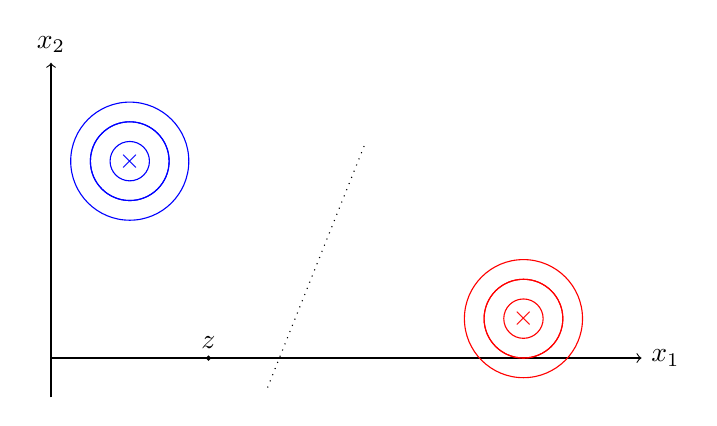
\begin{tikzpicture}[scale=0.5]
				\draw[->] (0,0) -- (15,0) node[right] {$x_1$};
				\draw[->] (0,-1) -- (0,7.5) node[above] {$x_2$};
				
				\node[blue] at (2,5) {$\times$};
				\draw[blue] (2,5) circle (0.5);
				\draw[blue] (2,5) circle (1);
				\draw[blue] (2,5) circle (1.5);
				\draw[blue] (2,5) circle (1);
				
				\node[red] at (12,1) {$\times$};
				\draw[red] (12,1) circle (0.5);
				\draw[red] (12,1) circle (1);
				\draw[red] (12,1) circle (1.5);
				\draw[red] (12,1) circle (1);
				
				\draw[dotted] (5.5,-0.75) -- (8,5.5);
				\draw[fill=black] (4,0) circle (0.05) node[above] {$z$};
			\end{tikzpicture}
		\end{center}
		\item Analog zu (a) ergibt sich
		\begin{align}
			\hat{\Sigma}^{-1} &= \begin{pmatrix}
				\frac{1}{4} & 0 \\ 0 & 1
			\end{pmatrix} \notag \\
			a &= \hat{\Sigma}^{-1}(\bar{x}^{C_1} - \bar{x}^{C_2}) = (-2.5,4)' \notag \\
			t &= a'\frac{\bar{x}^{C_1} + \bar{x}^{C_2}}{2} = -5.5 \notag
		\end{align}
		Um ein Objekt in Klasse 1 einzuordnen, muss gelten $-2.5x_1 + 4x_2 > -5.5$. Die diskriminierende Kurve lautet also: $x_2 = -\frac{11}{8} + \frac{5}{8}x_1$. Tatsächlich wird der Punkt $z$  Klasse 2 zugeordnet.
		\begin{center}
			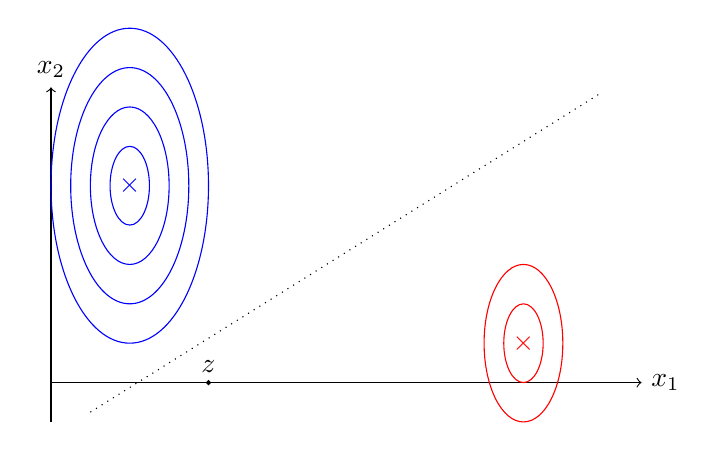
\begin{tikzpicture}[scale=0.5]
				\draw[->] (0,0) -- (15,0) node[right] {$x_1$};
				\draw[->] (0,-1) -- (0,7.5) node[above] {$x_2$};
				
				\node[blue] at (2,5) {$\times$};
				\draw[blue] (2,5) ellipse (0.5 and 1);
				\draw[blue] (2,5) ellipse (1 and 2);
				\draw[blue] (2,5) ellipse (1.5 and 3);
				\draw[blue] (2,5) ellipse (2 and 4);
				
				\node[red] at (12,1) {$\times$};
				\draw[red] (12,1) ellipse (0.5 and 1);
				\draw[red] (12,1) ellipse (1 and 2);
				
				\draw[dotted] (1,-0.75) -- (14,7.375);
				\draw[fill=black] (4,0) circle (0.05) node[above] {$z$};
			\end{tikzpicture}
		\end{center}
		\item Analog zu (a) ergibt sich
		\begin{align}
			\hat{\Sigma}^{-1} &= \begin{pmatrix}
				\frac{1}{3} & -\frac{1}{3} \\ -\frac{1}{3} & \frac{4}{3}
			\end{pmatrix} \notag \\
			a &= \hat{\Sigma}^{-1}(\bar{x}^{C_1} - \bar{x}^{C_2}) = \left(-\frac{14}{3},\frac{26}{3}\right)' \notag \\
			t &= a'\frac{\bar{x}^{C_1} + \bar{x}^{C_2}}{2} = -\frac{20}{3} \notag
		\end{align}
		Um ein Objekt in Klasse 1 einzuordnen, muss gelten $-\frac{14}{3}x_1 + \frac{26}{3}x_2 > -\frac{20}{3}$. Die diskriminierende Kurve lautet also: $x_2 = -\frac{10}{13} + \frac{7}{13}x_1$. Tatsächlich wird der Punkt $z$  Klasse 2 zugeordnet.
		\begin{center}
			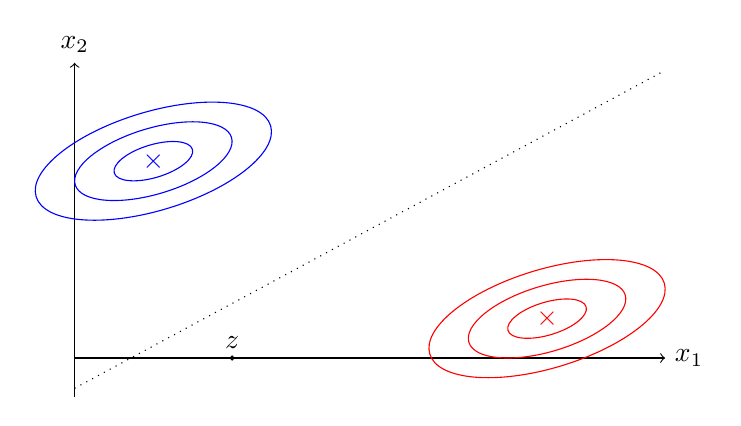
\begin{tikzpicture}[scale=0.5]
				\draw[->] (0,0) -- (15,0) node[right] {$x_1$};
				\draw[->] (0,-1) -- (0,7.5) node[above] {$x_2$};
				
				\node[blue] at (2,5) {$\times$};
				\draw[blue,rotate around={-73.154:(2,5)}] (2,5) ellipse (0.417 and 1.0372);
				\draw[blue,rotate around={-73.154:(2,5)}] (2,5) ellipse (0.835 and 2.0743);
				\draw[blue,rotate around={-73.154:(2,5)}] (2,5) ellipse (1.2525 and 3.1115);
				
				\node[red] at (12,1) {$\times$};
				\draw[red,rotate around={-73.154:(12,1)}] (12,1) ellipse (0.417 and 1.0372);
				\draw[red,rotate around={-73.154:(12,1)}] (12,1) ellipse (0.835 and 2.0743);
				\draw[red,rotate around={-73.154:(12,1)}] (12,1) ellipse (1.2525 and 3.1115);
				
				\draw[dotted] (0,-10/13) -- (15,95/13);
				\draw[fill=black] (4,0) circle (0.05) node[above] {$z$};
			\end{tikzpicture}
		\end{center}
	\end{enumerate}

	\section*{Aufgabe 2}
	\begin{enumerate}[label=(\alph*)]
		\item Diagramm
		\begin{center}
			\begin{tikzpicture}
				\begin{axis}[
					xmin=-2, xmax=2, xlabel=$x$,
					ymin=0, ymax=1.5, ylabel=$f(x)$,
					samples=400,
					axis x line=middle,
					axis y line=middle,
					domain=-2:2,
					]
					\addplot[mark=none,smooth,blue] {1-abs(x)};
					\addplot[mark=none,smooth,red] {1-abs(x-0.5)};
					
				\end{axis}
			\end{tikzpicture}
		\end{center}
		\item Für den Fall gleicher Fehlklassifikationskosten und gleicher a-priori-Wahrscheinlichkeiten gilt
		\begin{align}
			R_1 &= \left\lbrace x\mid f_1(x) \ge f_2(x)\right\rbrace \notag \\
			R_2 &= \left\lbrace x\mid f_1(x) < f_2(x)\right\rbrace \notag
		\end{align}
		Wir müssen also den Schnittpunkt der beiden Dichtefunktionen bestimmen.
		\begin{align}
			1-\vert x\vert &= 1- \vert x-0.5\vert \notag \\
			\vert x\vert &= \vert x-0.5\vert \notag
		\end{align}
		Fallunterscheidung: Entweder ist $x\ge 0$ oder nicht:
		\begin{itemize}
			\item $x\ge 0$:
			\begin{align}
				x = \vert x-0.5\vert \notag
			\end{align}
			Fallunterscheidung: Entweder ist $x\ge 0.5$ oder nicht:
			\begin{itemize}
				\item $x\ge 0.5$:
				\begin{align}
					x &= x-0.5 \notag \\
					0 &= -0.5 \Rightarrow \text{Widerspruch} \notag
				\end{align}
				\item $x<0.5$:
				\begin{align}
					x &= -(x-0.5) \notag \\
					x &= -x + 0.5 \notag \\
					2x &= 0.5 \notag \\
					x &= 0.25 \notag
				\end{align}
			\end{itemize}
			\item $x < 0$:
			\begin{align}
				-x = \vert x-0.5\vert \notag
			\end{align}
			Fallunterscheidung: Entweder ist $x\ge 0.5$ oder nicht:
			\begin{itemize}
				\item $x\ge 0.5$: Widerspruch, da $x<0$ schon angenommen ist
				\item $x<0.5$:
				\begin{align}
					-x &= -(x-0.5) \notag \\
					x &= x-0.5 \notag \\
					0 &= -0.5 \Rightarrow\text{Widerspruch} \notag
				\end{align}
			\end{itemize}
		\end{itemize}
		Der Schnittpunkt der beiden Dichten ist also bei $x=\frac{1}{4}$. Damit ist
		\begin{align}
			R_1 &= \left[-1,\frac{1}{4}\right] \notag \\
			R_2 &= \left(\frac{1}{4},\frac{3}{2}\right] \notag
		\end{align}
		\item Jetzt lauten die Klassifikationsregionen
		\begin{align}
			R_1 &= \left\lbrace x\mid f_1(x)\cdot 0.2 \ge f_2(x)\cdot 0.8\right\rbrace \notag \\
			R_2 &= \left\lbrace x\mid f_1(x)\cdot 0.2 < f_2(x)\cdot 0.8\right\rbrace \notag
		\end{align}
		Wir interessieren uns wieder für den Schnittpunkt von $0.2\cdot f_1(x)$ und $0.8\cdot f_2(x)$. Die Rechnung ist ziemlich analog wie oben, der Schnittpunkt ist bei $x=-\frac{1}{3}$.
		\begin{center}
			\begin{tikzpicture}
				\begin{axis}[
					xmin=-2, xmax=2, xlabel=$x$,
					ymin=0, ymax=1.5, ylabel=$f(x)$,
					samples=400,
					axis x line=middle,
					axis y line=middle,
					domain=-2:2,
					]
					\addplot[mark=none,smooth,blue] {0.2-0.2*abs(x)};
					\addplot[mark=none,smooth,red] {0.8-0.8*abs(x-0.5)};
					
				\end{axis}
			\end{tikzpicture}
		\end{center}
		Die Regionen sind also
		\begin{align}
			R_1 &= \left[-1,-\frac{1}{3}\right] \notag \\
			R_2 &= \left(-\frac{1}{3},\frac{3}{2}\right] \notag
		\end{align}
		\item Jetzt lauten die Klassifikationsregionen
		\begin{align}
			R_1 &= \left\lbrace x\mid f_1(x)\cdot 0.2 \ge f_2(x)\cdot 0.8\cdot\frac{0.5}{1}\right\rbrace \notag \\
			R_2 &= \left\lbrace x\mid f_1(x)\cdot 0.2 < f_2(x)\cdot 0.8\cdot\frac{0.5}{1}\right\rbrace \notag
		\end{align}
		Wir interessieren uns wieder für den Schnittpunkt von $0.2\cdot f_1(x)$ und $0.4\cdot f_2(x)$. Die Rechnung ist ziemlich analog wie oben, der Schnittpunkt ist bei $x=0$.
		\begin{center}
			\begin{tikzpicture}
				\begin{axis}[
					xmin=-2, xmax=2, xlabel=$x$,
					ymin=0, ymax=1.5, ylabel=$f(x)$,
					samples=400,
					axis x line=middle,
					axis y line=middle,
					domain=-2:2,
					]
					\addplot[mark=none,smooth,blue] {0.2-0.2*abs(x)};
					\addplot[mark=none,smooth,red] {0.4-0.4*abs(x-0.5)};
					
				\end{axis}
			\end{tikzpicture}
		\end{center}
		Die Regionen sind also
		\begin{align}
			R_1 &= \left[-1,0\right] \notag \\
			R_2 &= \left(0,\frac{3}{2}\right] \notag
		\end{align}
	\end{enumerate}

	\section*{Berechnung der Höhenlinien}
	Weil es nicht ganz einfach ist, die Höhenlinien auszurechnen, hier noch mal eine detaillierte Erklärung anhand $\hat{\Sigma}$ von (b): Die Eigenwerte von $\hat{\Sigma}^{-1}$ sind $\lambda_1=1$ und $\lambda_2=\frac{1}{4}$ und die Eigenvektoren \textcolor{red}{$v_1=(1,0)'$} und \textcolor{red}{$v_2=(0,1)'$}. Wir wählen als Abstand $d=1$ und damit sind die Achsenlängen der Ellipsen der Höhenlinien
	\begin{align}
		\textcolor{green!80!black}{a} &= \sqrt{\frac{1^2}{1}} = 1 \notag \\
		\textcolor{green!80!black}{b} &= \sqrt{\frac{1^2}{0.25}} = 2 \notag
	\end{align}
	Zeichnen wir das ganze ein.
	\begin{center}
		\begin{tikzpicture}
			\draw[->] (0,0) -- (5,0) node[right] {$x_1$};
			\draw[->] (0,0) -- (0,7.5) node[above] {$x_2$};
			
			\node[blue] at (2,5) {$\times$};
			\draw[dotted] (2,0) node[below] {2} -- (2,5) -- (0,5) node[left] {5};
			
			\draw[->,red] (2,5) to node[midway, right] {$v_2$} (2,6);
			\draw[dashed,red] (2,5) -- (2,7.5);
			\draw[->,red] (2,5) to node[midway, above] {$v_1$} (3,5);
			\draw[dashed,red] (2,5) -- (3.5,5);
			\draw[blue] (2,5) ellipse (1 and 2);
			
			\draw [decorate,decoration={brace,amplitude=10pt},green!80!black] (2,5) -- (2,7) node [green!80!black,midway,xshift=-0.5cm] {$a$};
			\draw [decorate,decoration={brace,amplitude=10pt,mirror},green!80!black]
			(2,5) -- (3,5) node [green!80!black,midway,yshift=-0.6cm] {$b$};
		\end{tikzpicture}
	\end{center}
\end{document}